\documentclass[a4paper,11pt]{ctexart}
\title{\Huge\textbf{Homework}}
\author{Yourname}
\usepackage{graphicx}
\usepackage{fancyhdr}
\pagestyle{fancy}
\lhead{
\includegraphics[scale=0.1]{logo.png}}  %在此处插入logo.pdf图片 图片靠左
%\lhead{
\includegraphics[scale=0.1]{wy.jpg}} %if you prefer to use logo of weiyang
\chead{} % 页眉中间位置内容
\rightmark 
\usepackage{multirow}
\usepackage{amsmath}
\usepackage[colorlinks,linkcolor=red]{hyperref}
\usepackage{soul}
\usepackage{fontspec}
\usepackage[table,xcdraw]{xcolor}
\usepackage{amssymb,xtab}
\usepackage{url}
\usepackage[all,cmtip]{xy}
\usepackage{fontspec,xltxtra,xunicode,amsmath,amsthm,amssymb,mathrsfs,stmaryrd,eucal}


 \usepackage{color}

 \usepackage{yhmath}

\usepackage{graphicx}
\usepackage{amssymb}
\usepackage{bm}

\usepackage{ctex}
\graphicspath{{photo/}}

%定理环境
\usepackage{hyperref}
\usepackage{indentfirst}
\usepackage{url}


\newtheorem{thm}{定理}[section]
\newtheorem{lem}[thm]{引理}
\newtheorem{prop}[thm]{命题}
\newtheorem{propdefn}[thm]{命题-定义}
\newtheorem{cor}[thm]{推论}
\newtheorem{alg}[thm]{Algorithm}
\newtheorem{conj}[thm]{Conjecture}
\newtheorem{ques}[thm]{问题}
\newtheorem{prop-defn}[thm]{Proposition-Definition}
\newtheorem{clm}[thm]{Claim}
%\theoremstyle{definition}
\newtheorem{defn}[thm]{定义}
\newtheorem{const}[thm]{Construction}
\newtheorem{exam}[thm]{例}
\newtheorem{rem}[thm]{注}
\newtheorem{warn}[thm]{Warning}
%\theoremstyle{remark}
\newtheorem{thesis}[thm]{Thesis}


\newtheorem{notation}[thm]{记号}


\renewcommand{\proofname}{证明:}


\begin{document}
\maketitle

\begin{figure}[b]
    \centering
\begin{minipage}[t]{0.48\textwidth}
    \centering
    
\includegraphics[scale=0.6]{logo.png}    
\end{minipage}
\begin{minipage}[t]{0.48\textwidth}
    \centering
    
\includegraphics[scale=1.55]{wy.jpg}    
\end{minipage}

\end{figure}

\newpage
\begin{abstract}
    This is your abstract(if you really have an abstract). 
\end{abstract}
\newpage
    \tableofcontents
\section{problem 1}
\begin{thm}[勾股定理]
    如果$a$,$b$,$c$为直角三角形的三边长,那么有:
    \[a^2+b^2=c^2
    \]
\end{thm}
\begin{proof}
    如图,这几乎是显然的。
    \begin{figure}[h]
        \centering
        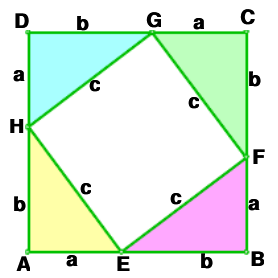
\includegraphics{gougu.png}
    \end{figure}
\end{proof}
\end{document}